\section{Conditional calibration: full diagnostic record}\label{app:audit12}


The complete reference shows material count, temporal and spatial discrepancies for the original frozen Omori continuous (OC) forecast, alongside some ordinary-looking diagnostics. It does not support a broad adequacy claim. This is a retrospective, exploratory, fixed-state conditional check of 315 already inspected targets: 79, 167 and 69 in [2011,2016), [2016,2021) and [2021,2026). No parameters or nuisance choices were refitted.

The target remains original OC, with its density-weighted rational offspring spatial kernel and smooth background. Thread01's separately fitted optimized smooth inverse-power ETAS comparator (EP) exceeded OC by 51.051204763 pooled joint nats. That relative predictive comparison did not replace the frozen target, and it does not establish EP's adequacy. These diagnostics do not calibrate EP.

\subsection{Reference and interpretation}

Each origin has 999 complete dependent branching-future paths, conditional on its own original prehistory and fitted/nuisance state. All 2,997 planned paths are complete; failed and unknown counts are both zero. Simulated events can generate descendants. Sequential observed scores use every strictly earlier admissible event. The issue-frozen NHPP is a different forecast object and has no empirical arm here. The observed-path exposure is a realised predictable compensator, not a Poisson future-count mean.

For each coordinate, the complete tables report the observed value $y$, inclusive counts $L=\#\{Y_b\leq y\}$ and $H=\#\{Y_b\geq y\}$, ties, its insertion interval and the supplied empirical reference interval. With $B=999$ complete paths, the insertion interval is
\[
 \left[\frac{1+\#\{Y_b<y\}}{1000},\;
       \frac{1+\#\{Y_b\leq y\}}{1000}\right].
\]
The inclusive lower and upper tails are $(1+L)/1000$ and $(1+H)/1000$. Resolution is $0.001$. A boundary rank is a finite comparison, not a zero probability or an exact population tail probability. Ties can make insertion intervals wide. All $84$ coordinates per origin form one descriptive collection; individual tails are not separate unadjusted discoveries, and no omnibus significance test is asserted. Reference intervals describe simulated catalogues, not confidence intervals for fitted parameters or model validity.

The coordinate \texttt{immigrant\_exposure} is marked \emph{fixed} in every table: its reference variance is zero by construction and it is not a stochastic adequacy diagnostic. Adding it to trigger exposure produces total exposure, so the latter two insertion intervals are duplicates within an origin. The full accounting vector is preserved, but its length must not be interpreted as the number of independent tests.

\subsection{What the complete vector shows}

Early origin: count 79 is below all 999 simulated counts (L=0,H=999,ties=0; insertion 0.001), with supplied count reference interval 121 to 453. Exposure 114.54932024184329 and trigger exposure 38.82182627332281 are also below all references. Count minus exposure is -35.54932024184329 (L=10,H=989; insertion 0.011). Gap KS 0.22224496322920195 and gap serial statistic 0.025311536051231393 both exceed every reference. Spatial Rosenblatt KS 0.16733517789142327 exceeds every reference; location dimensionless mean 2.4494637138726643 is below all references and variance 10.653917170486158 is above all. Yet time event-logsum insertion is 0.583, censored tail 0.111 and within-cell absolute maximum 0.187. The second year count 30 has insertion interval [0.370,0.409], with 39 ties. This is not uniformly poor on every coordinate.

Middle origin: total count 167 looks ordinary in its reference (L=711,H=296,ties=8; insertion [0.704,0.712], supplied count interval 90 to 398). Balance -4.373290651999895 has insertion 0.391. This total hides subblock concentration: yearly counts are 12,4,8,116,27; subblock balance maximum 0.6836875842626084 has L=997,H=2 and insertion 0.998. The fourth year's balance is +25.931179418686256 (insertion 0.998). Gap KS 0.15088891163993823 has H=8; serial 0.05049115130656217 exceeds all 999. Spatial KS 0.16932136137657972 has H=4, cross statistic 0.027677364202278305 exceeds all 999, and cell-mass residual maximum 1.278459418085198 has H=11. Conditional-location logscore insertion 0.364, within-cell density score 0.312, terminal tail 0.237 and within-cell absolute maximum 0.341 illustrate ordinary-looking components alongside those discrepancies.

Late origin: count 69 lies toward the low end (L=27,H=979,ties=7; insertion [0.021,0.028], supplied interval 69 to 279). Exposure 82.98011402768624 has insertion 0.012, while balance -13.980114027686241 has insertion 0.110. Gap KS 0.0881227829042357 has insertion 0.676, spatial KS 0.1129696501693383 has insertion 0.810 and terminal tail 1.586732938471152 has insertion 0.700. However serial statistic 0.02308692546525953 has H=2 (insertion 0.998), spatial cross statistic 0.021671079327220788 has H=8 (0.992), and dimensionless location variance 12.30394407102264 exceeds all references. Within-cell absolute maximum has insertion 0.499. A reasonable marginal shape statistic therefore does not settle dependence or concentration.

Across the descriptive cell tables, cell 4 counts are 15,7,8 against conditional expected allocations 23.493716546234523,16.132286198379887,14.770085109767768. These allocations sum conditional probabilities at the observed event times; they are not unconditional count means. Their count-minus-allocation values have insertion ranks 0.074,0.029,0.047. Other cells differ in direction: middle cell 7 count 124 has insertion 0.992, and late cell 3 count-minus-allocation +5.305104300093006 has insertion 0.991. Empty cells often tie extensively: early cell 8 count zero has 562 ties and insertion [0.001,0.563], so its lower endpoint alone is misleading.

Raw total log scores depend on the number of events and the score measure. For example early joint and location log scores exceed all reference totals while count is below all references; this is not evidence of adequate probabilities. Dimensionless location summaries, allocation residuals and spatial transforms provide complementary information. Immigrant exposure is deterministic within each fixed state: all 999 references tie at 75.72749396852048,65.12820992122843,51.19150695498898 respectively. Its [0.001,1.000] insertion interval is expected by construction, not an adequacy result. Mark totals also vary with count and do not independently validate the mark or productivity recipe.

\subsection{Independent computational audit and limits}

The independent campaign audit passed identity/hash/status/seed checks and all-path raw count, mark and temporal-exposure checks for 2,997 paths. The full 84-coordinate raw diagnostic replay was sampled: indices 0,499,998 in each origin, nine complete paths. Maximum sampled absolute score difference was 2.2737367544323206e-12 nats (gate 1e-4); maximum non-score difference 3.410605131648481e-13 and spatial CDF difference 6.217248937900877e-15. This does not mean all 2,997 paths received full-vector independent replay. Original observed reconstructions are separately bound by the approved report's execution and oracle receipt hashes. Numerical agreement checks implementation; it does not validate the forecast's scientific adequacy.

The fitted state, training history and nuisance choices are fixed; fitting, selection, measurement and catalogue-revision uncertainty are excluded. Later observed training histories include earlier target periods, so independent per-origin simulations do not define a coherent cross-origin joint null. Cross-window patterns and any pooled quantities remain descriptive. There is no event-iid confidence interval, Wilks inference, causal triggering conclusion, untouched holdout, general calibration or validation claim. Heavy-tailed productivity has infinite second moment under the fixed mark recipe; normal/CLT count arguments are not used. Terminal exposure is censored survival information, never an added completed gap. No observed rounding model, post-observation metric choice or seed extension was introduced.

\subsection{Evidence and transition}

The sole numerical reporting input is approved scalar report, SHA256 \nolinkurl{731a4a1481fc4dee9297a8cccba6012f1096803f5551171501f22bbd64233f93}. Definitions are in frozen protocol, fixed methods and independent design. Audit evidence is campaign audit. The complete HTML table and the appendix cover all 252 coordinates. Rendering-only revised rank figures are early, middle, late; the JSON, rather than plotted glyphs, is authoritative.

The subsequent completed score-concentration and catalogue-robustness study retained these discrepant and ordinary-looking diagnostics. Its exact annual accounting preserved every event history and full exposure before the separately admitted higher-threshold sensitivity. Those completed results appear in Chapter~\ref{ch:external}; the frozen OC target was retained by that follow-on.

\subsection{Complete coordinate appendix}

Years are chronological, zero-based within each five-year window. Cells 0 to 8 are row-major latitude then longitude. Values are rounded for display; the approved JSON retains full precision. Every row has planned=complete=999 and failed/unknown=0. RI denotes the supplied empirical reference interval; it is not an inferential acceptance band.

\subsubsection{california\_\allowbreak{}fold\_\allowbreak{}0}

\begingroup\scriptsize\setlength{\tabcolsep}{2pt}\renewcommand{\arraystretch}{1.12}
\begin{longtable}{@{}>{\raggedright\arraybackslash}p{0.2100\textwidth}>{\raggedright\arraybackslash}p{0.1200\textwidth}>{\raggedright\arraybackslash}p{0.0400\textwidth}>{\raggedright\arraybackslash}p{0.0400\textwidth}>{\raggedright\arraybackslash}p{0.0400\textwidth}>{\raggedright\arraybackslash}p{0.1400\textwidth}>{\raggedright\arraybackslash}p{0.2400\textwidth}@{}}
\toprule
{}Coordinate & Observed & L & H & Ties & Insertion interval & RI \\
\midrule\endfirsthead
\toprule
Coordinate & Observed & L & H & Ties & Insertion interval & RI \\
\midrule\endhead
\midrule\multicolumn{7}{r}{\emph{Continued on next page}}\\
\endfoot
\bottomrule\endlastfoot
{}count & 79 & 0 & 999 & 0 & [0.001, 0.001] & [121, 453] \\
{}exposure & 114.549 & 0 & 999 & 0 & [0.001, 0.001] & [135.568, 486.759] \\
{}immigrant\_\allowbreak{}exposure (fixed) & 75.7275 & 999 & 999 & 999 & [0.001, 1.000] & [75.7275, 75.7275] \\
{}trigger\_\allowbreak{}exposure & 38.8218 & 0 & 999 & 0 & [0.001, 0.001] & [59.8403, 411.031] \\
{}count\_\allowbreak{}minus\_\allowbreak{}exposure & -35.5493 & 10 & 989 & 0 & [0.011, 0.011] & [-27.6883, 30.0604] \\
{}time\_\allowbreak{}event\_\allowbreak{}logsum & -176.459 & 582 & 417 & 0 & [0.583, 0.583] & [-286.513, 722.925] \\
{}timing\_\allowbreak{}logscore & -291.008 & 832 & 167 & 0 & [0.833, 0.833] & [-457.245, 177.529] \\
{}location\_\allowbreak{}logscore & -816.442 & 999 & 0 & 0 & [1.000, 1.000] & [-3711.06, -1114.36] \\
{}mark\_\allowbreak{}logscore & 6.45748 & 995 & 4 & 0 & [0.996, 0.996] & [-99.9643, -0.728886] \\
{}joint\_\allowbreak{}logscore & -1100.99 & 999 & 0 & 0 & [1.000, 1.000] & [-3577.51, -1463.15] \\
{}zone\_\allowbreak{}logscore & -74.7927 & 993 & 6 & 0 & [0.994, 0.994] & [-165.841, -82.9881] \\
{}cell\_\allowbreak{}given\_\allowbreak{}zone\_\allowbreak{}logscore & -42.5394 & 989 & 10 & 0 & [0.990, 0.990] & [-118.87, -46.1742] \\
{}within\_\allowbreak{}cell\_\allowbreak{}density\_\allowbreak{}logscore & -699.11 & 999 & 0 & 0 & [1.000, 1.000] & [-3254.52, -969.257] \\
{}subblock\_\allowbreak{}balance\_\allowbreak{}max & 0.461367 & 960 & 39 & 0 & [0.961, 0.961] & [0.0994411, 0.481693] \\
{}gap\_\allowbreak{}ks & 0.222245 & 999 & 0 & 0 & [1.000, 1.000] & [0.0301227, 0.11125] \\
{}gap\_\allowbreak{}serial & 0.0253115 & 999 & 0 & 0 & [1.000, 1.000] & [-0.0125117, 0.012663] \\
{}censored\_\allowbreak{}tail & 0.363034 & 110 & 889 & 0 & [0.111, 0.111] & [0.172443, 4.35742] \\
{}spatial\_\allowbreak{}rosenblatt\_\allowbreak{}ks\_\allowbreak{}max & 0.167335 & 999 & 0 & 0 & [1.000, 1.000] & [0.0369932, 0.120491] \\
{}spatial\_\allowbreak{}rosenblatt\_\allowbreak{}cross\_\allowbreak{}abs & 0.0136967 & 979 & 20 & 0 & [0.980, 0.980] & [0.000180014, 0.0134149] \\
{}cell\_\allowbreak{}mass\_\allowbreak{}residual\_\allowbreak{}max & 0.944775 & 940 & 59 & 0 & [0.941, 0.941] & [0.273419, 1.25152] \\
{}location\_\allowbreak{}dimensionless\_\allowbreak{}log\_\allowbreak{}mean & 2.44946 & 0 & 999 & 0 & [0.001, 0.001] & [3.22345, 5.12333] \\
{}location\_\allowbreak{}dimensionless\_\allowbreak{}log\_\allowbreak{}variance & 10.6539 & 999 & 0 & 0 & [1.000, 1.000] & [5.42532, 8.42119] \\
{}within\_\allowbreak{}cell\_\allowbreak{}dimensionless\_\allowbreak{}absmax & 6.18894 & 186 & 813 & 0 & [0.187, 0.187] & [6.05597, 6.93833] \\
{}within\_\allowbreak{}cell\_\allowbreak{}dimensionless\_\allowbreak{}sum & 137.844 & 0 & 999 & 0 & [0.001, 0.001] & [280.681, 1543.46] \\
{}year\_\allowbreak{}count[0] & 14 & 17 & 988 & 6 & [0.012, 0.018] & [16, 137] \\
{}year\_\allowbreak{}count[1] & 30 & 408 & 630 & 39 & [0.370, 0.409] & [14, 102] \\
{}year\_\allowbreak{}count[2] & 13 & 16 & 990 & 7 & [0.010, 0.017] & [14, 121] \\
{}year\_\allowbreak{}count[3] & 12 & 19 & 986 & 6 & [0.014, 0.020] & [14, 152] \\
{}year\_\allowbreak{}count[4] & 10 & 2 & 998 & 1 & [0.002, 0.003] & [15, 137] \\
{}year\_\allowbreak{}exposure[0] & 22.3768 & 7 & 992 & 0 & [0.008, 0.008] & [23.4745, 132.734] \\
{}year\_\allowbreak{}exposure[1] & 30.6867 & 382 & 617 & 0 & [0.383, 0.383] & [22.4225, 104.079] \\
{}year\_\allowbreak{}exposure[2] & 20.8572 & 4 & 995 & 0 & [0.005, 0.005] & [22.4249, 111.59] \\
{}year\_\allowbreak{}exposure[3] & 21.2066 & 10 & 989 & 0 & [0.011, 0.011] & [22.4176, 150.938] \\
{}year\_\allowbreak{}exposure[4] & 19.4221 & 0 & 999 & 0 & [0.001, 0.001] & [22.9658, 124.594] \\
{}year\_\allowbreak{}count\_\allowbreak{}minus\_\allowbreak{}exposure[0] & -8.3768 & 65 & 934 & 0 & [0.066, 0.066] & [-10.4097, 14.7207] \\
{}year\_\allowbreak{}count\_\allowbreak{}minus\_\allowbreak{}exposure[1] & -0.686685 & 470 & 529 & 0 & [0.471, 0.471] & [-10.1202, 14.0157] \\
{}year\_\allowbreak{}count\_\allowbreak{}minus\_\allowbreak{}exposure[2] & -7.85718 & 88 & 911 & 0 & [0.089, 0.089] & [-10.827, 14.85] \\
{}year\_\allowbreak{}count\_\allowbreak{}minus\_\allowbreak{}exposure[3] & -9.2066 & 64 & 935 & 0 & [0.065, 0.065] & [-11.3972, 14.9039] \\
{}year\_\allowbreak{}count\_\allowbreak{}minus\_\allowbreak{}exposure[4] & -9.42206 & 40 & 959 & 0 & [0.041, 0.041] & [-10.3287, 17.6716] \\
{}cell\_\allowbreak{}count[0] & 1 & 898 & 288 & 187 & [0.712, 0.899] & [0, 5] \\
{}cell\_\allowbreak{}count[1] & 5 & 325 & 763 & 89 & [0.237, 0.326] & [1, 41] \\
{}cell\_\allowbreak{}count[2] & 39 & 169 & 852 & 22 & [0.148, 0.170] & [27, 178] \\
{}cell\_\allowbreak{}count[3] & 2 & 260 & 854 & 115 & [0.146, 0.261] & [0, 23] \\
{}cell\_\allowbreak{}count[4] & 15 & 0 & 999 & 0 & [0.001, 0.001] & [35, 218] \\
{}cell\_\allowbreak{}count[5] & 2 & 12 & 994 & 7 & [0.006, 0.013] & [3, 42] \\
{}cell\_\allowbreak{}count[6] & 7 & 660 & 414 & 75 & [0.586, 0.661] & [1, 31] \\
{}cell\_\allowbreak{}count[7] & 8 & 227 & 834 & 62 & [0.166, 0.228] & [4, 56] \\
{}cell\_\allowbreak{}count[8] & 0 & 562 & 999 & 562 & [0.001, 0.563] & [0, 5] \\
{}cell\_\allowbreak{}conditional\_\allowbreak{}expected[0] & 0.264795 & 22 & 977 & 0 & [0.023, 0.023] & [0.266605, 2.60346] \\
{}cell\_\allowbreak{}conditional\_\allowbreak{}expected[1] & 3.39765 & 0 & 999 & 0 & [0.001, 0.001] & [4.20337, 38.4866] \\
{}cell\_\allowbreak{}conditional\_\allowbreak{}expected[2] & 34.7782 & 49 & 950 & 0 & [0.050, 0.050] & [32.7803, 180.086] \\
{}cell\_\allowbreak{}conditional\_\allowbreak{}expected[3] & 2.42206 & 0 & 999 & 0 & [0.001, 0.001] & [2.77168, 21.7863] \\
{}cell\_\allowbreak{}conditional\_\allowbreak{}expected[4] & 23.4937 & 0 & 999 & 0 & [0.001, 0.001] & [39.125, 218.36] \\
{}cell\_\allowbreak{}conditional\_\allowbreak{}expected[5] & 5.33786 & 0 & 999 & 0 & [0.001, 0.001] & [7.36546, 39.439] \\
{}cell\_\allowbreak{}conditional\_\allowbreak{}expected[6] & 3.11359 & 40 & 959 & 0 & [0.041, 0.041] & [3.00673, 27.2229] \\
{}cell\_\allowbreak{}conditional\_\allowbreak{}expected[7] & 5.78427 & 1 & 998 & 0 & [0.002, 0.002] & [7.40276, 53.2884] \\
{}cell\_\allowbreak{}conditional\_\allowbreak{}expected[8] & 0.407903 & 0 & 999 & 0 & [0.001, 0.001] & [0.483074, 4.0325] \\
{}cell\_\allowbreak{}exposure[0] & 0.558912 & 837 & 162 & 0 & [0.838, 0.838] & [0.321129, 2.05508] \\
{}cell\_\allowbreak{}exposure[1] & 5.71935 & 149 & 850 & 0 & [0.150, 0.150] & [4.99354, 37.8893] \\
{}cell\_\allowbreak{}exposure[2] & 43.1983 & 134 & 865 & 0 & [0.135, 0.135] & [37.6058, 176.193] \\
{}cell\_\allowbreak{}exposure[3] & 4.01574 & 317 & 682 & 0 & [0.318, 0.318] & [3.17289, 20.7453] \\
{}cell\_\allowbreak{}exposure[4] & 36.1404 & 0 & 999 & 0 & [0.001, 0.001] & [45.597, 209.277] \\
{}cell\_\allowbreak{}exposure[5] & 7.84627 & 2 & 997 & 0 & [0.003, 0.003] & [8.53853, 38.8116] \\
{}cell\_\allowbreak{}exposure[6] & 6.71515 & 666 & 333 & 0 & [0.667, 0.667] & [3.56374, 27.1171] \\
{}cell\_\allowbreak{}exposure[7] & 9.77314 & 103 & 896 & 0 & [0.104, 0.104] & [8.74061, 47.3811] \\
{}cell\_\allowbreak{}exposure[8] & 0.582052 & 0 & 999 & 0 & [0.001, 0.001] & [0.582164, 3.19678] \\
{}cell\_\allowbreak{}count\_\allowbreak{}minus\_\allowbreak{}conditional\_\allowbreak{}expected[0] & 0.735205 & 918 & 81 & 0 & [0.919, 0.919] & [-0.38687, 2.15471] \\
{}cell\_\allowbreak{}count\_\allowbreak{}minus\_\allowbreak{}conditional\_\allowbreak{}expected[1] & 1.60235 & 744 & 255 & 0 & [0.745, 0.745] & [-4.11639, 5.82373] \\
{}cell\_\allowbreak{}count\_\allowbreak{}minus\_\allowbreak{}conditional\_\allowbreak{}expected[2] & 4.22184 & 808 & 191 & 0 & [0.809, 0.809] & [-10.355, 9.62315] \\
{}cell\_\allowbreak{}count\_\allowbreak{}minus\_\allowbreak{}conditional\_\allowbreak{}expected[3] & -0.422056 & 473 & 526 & 0 & [0.474, 0.474] & [-3.21669, 4.60473] \\
{}cell\_\allowbreak{}count\_\allowbreak{}minus\_\allowbreak{}conditional\_\allowbreak{}expected[4] & -8.49372 & 73 & 926 & 0 & [0.074, 0.074] & [-11.0784, 10.7925] \\
{}cell\_\allowbreak{}count\_\allowbreak{}minus\_\allowbreak{}conditional\_\allowbreak{}expected[5] & -3.33786 & 139 & 860 & 0 & [0.140, 0.140] & [-5.78535, 6.84044] \\
{}cell\_\allowbreak{}count\_\allowbreak{}minus\_\allowbreak{}conditional\_\allowbreak{}expected[6] & 3.88641 & 940 & 59 & 0 & [0.941, 0.941] & [-3.31407, 5.27876] \\
{}cell\_\allowbreak{}count\_\allowbreak{}minus\_\allowbreak{}conditional\_\allowbreak{}expected[7] & 2.21573 & 748 & 251 & 0 & [0.749, 0.749] & [-5.47284, 6.7455] \\
{}cell\_\allowbreak{}count\_\allowbreak{}minus\_\allowbreak{}conditional\_\allowbreak{}expected[8] & -0.407903 & 571 & 428 & 0 & [0.572, 0.572] & [-0.680562, 2.20553] \\
{}cell\_\allowbreak{}count\_\allowbreak{}minus\_\allowbreak{}exposure[0] & 0.441088 & 782 & 217 & 0 & [0.783, 0.783] & [-0.369183, 2.33848] \\
{}cell\_\allowbreak{}count\_\allowbreak{}minus\_\allowbreak{}exposure[1] & -0.719352 & 442 & 557 & 0 & [0.443, 0.443] & [-4.47976, 7.52299] \\
{}cell\_\allowbreak{}count\_\allowbreak{}minus\_\allowbreak{}exposure[2] & -4.19828 & 332 & 667 & 0 & [0.333, 0.333] & [-14.4546, 18.9275] \\
{}cell\_\allowbreak{}count\_\allowbreak{}minus\_\allowbreak{}exposure[3] & -2.01574 & 198 & 801 & 0 & [0.199, 0.199] & [-3.20664, 6.01319] \\
{}cell\_\allowbreak{}count\_\allowbreak{}minus\_\allowbreak{}exposure[4] & -21.1404 & 7 & 992 & 0 & [0.008, 0.008] & [-15.7661, 19.7682] \\
{}cell\_\allowbreak{}count\_\allowbreak{}minus\_\allowbreak{}exposure[5] & -5.84627 & 32 & 967 & 0 & [0.033, 0.033] & [-6.13766, 8.00333] \\
{}cell\_\allowbreak{}count\_\allowbreak{}minus\_\allowbreak{}exposure[6] & 0.284852 & 614 & 385 & 0 & [0.615, 0.615] & [-3.39293, 6.60789] \\
{}cell\_\allowbreak{}count\_\allowbreak{}minus\_\allowbreak{}exposure[7] & -1.77314 & 367 & 632 & 0 & [0.368, 0.368] & [-6.5223, 9.49155] \\
{}cell\_\allowbreak{}count\_\allowbreak{}minus\_\allowbreak{}exposure[8] & -0.582052 & 571 & 428 & 0 & [0.572, 0.572] & [-0.60909, 2.45499] \\
\end{longtable}\endgroup

\subsubsection{california\_\allowbreak{}fold\_\allowbreak{}1}

\begingroup\scriptsize\setlength{\tabcolsep}{2pt}\renewcommand{\arraystretch}{1.12}
\begin{longtable}{@{}>{\raggedright\arraybackslash}p{0.2100\textwidth}>{\raggedright\arraybackslash}p{0.1200\textwidth}>{\raggedright\arraybackslash}p{0.0400\textwidth}>{\raggedright\arraybackslash}p{0.0400\textwidth}>{\raggedright\arraybackslash}p{0.0400\textwidth}>{\raggedright\arraybackslash}p{0.1400\textwidth}>{\raggedright\arraybackslash}p{0.2400\textwidth}@{}}
\toprule
{}Coordinate & Observed & L & H & Ties & Insertion interval & RI \\
\midrule\endfirsthead
\toprule
Coordinate & Observed & L & H & Ties & Insertion interval & RI \\
\midrule\endhead
\midrule\multicolumn{7}{r}{\emph{Continued on next page}}\\
\endfoot
\bottomrule\endlastfoot
{}count & 167 & 711 & 296 & 8 & [0.704, 0.712] & [90, 398] \\
{}exposure & 171.373 & 766 & 233 & 0 & [0.767, 0.767] & [106.123, 397.718] \\
{}immigrant\_\allowbreak{}exposure (fixed) & 65.1282 & 999 & 999 & 999 & [0.001, 1.000] & [65.1282, 65.1282] \\
{}trigger\_\allowbreak{}exposure & 106.245 & 766 & 233 & 0 & [0.767, 0.767] & [40.9949, 332.589] \\
{}count\_\allowbreak{}minus\_\allowbreak{}exposure & -4.37329 & 390 & 609 & 0 & [0.391, 0.391] & [-24.363, 26.3737] \\
{}time\_\allowbreak{}event\_\allowbreak{}logsum & 326.504 & 963 & 36 & 0 & [0.964, 0.964] & [-265.132, 583.383] \\
{}timing\_\allowbreak{}logscore & 155.131 & 971 & 28 & 0 & [0.972, 0.972] & [-404.099, 178.164] \\
{}location\_\allowbreak{}logscore & -1377.21 & 363 & 636 & 0 & [0.364, 0.364] & [-3078.53, -854.24] \\
{}mark\_\allowbreak{}logscore & -15.039 & 680 & 319 & 0 & [0.681, 0.681] & [-81.6814, 1.52589] \\
{}joint\_\allowbreak{}logscore & -1237.12 & 948 & 51 & 0 & [0.949, 0.949] & [-3090.7, -1158.67] \\
{}zone\_\allowbreak{}logscore & -54.3512 & 998 & 1 & 0 & [0.999, 0.999] & [-141.063, -64.9197] \\
{}cell\_\allowbreak{}given\_\allowbreak{}zone\_\allowbreak{}logscore & -45.4093 & 852 & 147 & 0 & [0.853, 0.853] & [-94.9976, -36.3447] \\
{}within\_\allowbreak{}cell\_\allowbreak{}density\_\allowbreak{}logscore & -1277.45 & 311 & 688 & 0 & [0.312, 0.312] & [-2827.3, -745.781] \\
{}subblock\_\allowbreak{}balance\_\allowbreak{}max & 0.683688 & 997 & 2 & 0 & [0.998, 0.998] & [0.109334, 0.534276] \\
{}gap\_\allowbreak{}ks & 0.150889 & 991 & 8 & 0 & [0.992, 0.992] & [0.0338237, 0.133599] \\
{}gap\_\allowbreak{}serial & 0.0504912 & 999 & 0 & 0 & [1.000, 1.000] & [-0.0147719, 0.0133319] \\
{}censored\_\allowbreak{}tail & 0.616134 & 236 & 763 & 0 & [0.237, 0.237] & [0.187709, 4.19745] \\
{}spatial\_\allowbreak{}rosenblatt\_\allowbreak{}ks\_\allowbreak{}max & 0.169321 & 995 & 4 & 0 & [0.996, 0.996] & [0.0419072, 0.13574] \\
{}spatial\_\allowbreak{}rosenblatt\_\allowbreak{}cross\_\allowbreak{}abs & 0.0276774 & 999 & 0 & 0 & [1.000, 1.000] & [0.00016408, 0.0154671] \\
{}cell\_\allowbreak{}mass\_\allowbreak{}residual\_\allowbreak{}max & 1.27846 & 988 & 11 & 0 & [0.989, 0.989] & [0.290536, 1.12216] \\
{}location\_\allowbreak{}dimensionless\_\allowbreak{}log\_\allowbreak{}mean & 4.53739 & 906 & 93 & 0 & [0.907, 0.907] & [3.02673, 5.1304] \\
{}location\_\allowbreak{}dimensionless\_\allowbreak{}log\_\allowbreak{}variance & 8.76988 & 976 & 23 & 0 & [0.977, 0.977] & [5.13867, 8.72968] \\
{}within\_\allowbreak{}cell\_\allowbreak{}dimensionless\_\allowbreak{}absmax & 6.21235 & 340 & 659 & 0 & [0.341, 0.341] & [6.00424, 6.92997] \\
{}within\_\allowbreak{}cell\_\allowbreak{}dimensionless\_\allowbreak{}sum & 488.361 & 732 & 267 & 0 & [0.733, 0.733] & [205.4, 1400.6] \\
{}year\_\allowbreak{}count[0] & 12 & 71 & 952 & 24 & [0.048, 0.072] & [10, 90] \\
{}year\_\allowbreak{}count[1] & 4 & 1 & 999 & 1 & [0.001, 0.002] & [11, 84] \\
{}year\_\allowbreak{}count[2] & 8 & 8 & 995 & 4 & [0.005, 0.009] & [11, 101] \\
{}year\_\allowbreak{}count[3] & 116 & 985 & 14 & 0 & [0.986, 0.986] & [11, 82] \\
{}year\_\allowbreak{}count[4] & 27 & 514 & 525 & 40 & [0.475, 0.515] & [10, 78] \\
{}year\_\allowbreak{}exposure[0] & 18.2911 & 73 & 926 & 0 & [0.074, 0.074] & [17.2083, 89.5413] \\
{}year\_\allowbreak{}exposure[1] & 14.8072 & 0 & 999 & 0 & [0.001, 0.001] & [17.6359, 78.9419] \\
{}year\_\allowbreak{}exposure[2] & 17.9604 & 26 & 973 & 0 & [0.027, 0.027] & [17.9169, 106.21] \\
{}year\_\allowbreak{}exposure[3] & 90.0688 & 980 & 19 & 0 & [0.981, 0.981] & [18.2227, 78.0068] \\
{}year\_\allowbreak{}exposure[4] & 30.2459 & 643 & 356 & 0 & [0.644, 0.644] & [18.1292, 75.4797] \\
{}year\_\allowbreak{}count\_\allowbreak{}minus\_\allowbreak{}exposure[0] & -6.29107 & 100 & 899 & 0 & [0.101, 0.101] & [-9.38564, 12.2754] \\
{}year\_\allowbreak{}count\_\allowbreak{}minus\_\allowbreak{}exposure[1] & -10.8072 & 13 & 986 & 0 & [0.014, 0.014] & [-9.30059, 11.8518] \\
{}year\_\allowbreak{}count\_\allowbreak{}minus\_\allowbreak{}exposure[2] & -9.96035 & 15 & 984 & 0 & [0.016, 0.016] & [-9.09994, 12.8146] \\
{}year\_\allowbreak{}count\_\allowbreak{}minus\_\allowbreak{}exposure[3] & 25.9312 & 997 & 2 & 0 & [0.998, 0.998] & [-8.60357, 13.2453] \\
{}year\_\allowbreak{}count\_\allowbreak{}minus\_\allowbreak{}exposure[4] & -3.24589 & 323 & 676 & 0 & [0.324, 0.324] & [-9.7793, 11.4455] \\
{}cell\_\allowbreak{}count[0] & 0 & 717 & 999 & 717 & [0.001, 0.718] & [0, 4] \\
{}cell\_\allowbreak{}count[1] & 5 & 452 & 634 & 87 & [0.366, 0.453] & [1, 27] \\
{}cell\_\allowbreak{}count[2] & 17 & 13 & 988 & 2 & [0.012, 0.014] & [19, 134] \\
{}cell\_\allowbreak{}count[3] & 5 & 732 & 343 & 76 & [0.657, 0.733] & [0, 20] \\
{}cell\_\allowbreak{}count[4] & 7 & 0 & 999 & 0 & [0.001, 0.001] & [25, 191] \\
{}cell\_\allowbreak{}count[5] & 3 & 80 & 969 & 50 & [0.031, 0.081] & [2, 30] \\
{}cell\_\allowbreak{}count[6] & 4 & 454 & 626 & 81 & [0.374, 0.455] & [0, 27] \\
{}cell\_\allowbreak{}count[7] & 124 & 991 & 8 & 0 & [0.992, 0.992] & [2, 45] \\
{}cell\_\allowbreak{}count[8] & 2 & 947 & 129 & 77 & [0.871, 0.948] & [0, 4] \\
{}cell\_\allowbreak{}conditional\_\allowbreak{}expected[0] & 0.196435 & 0 & 999 & 0 & [0.001, 0.001] & [0.283822, 2.71701] \\
{}cell\_\allowbreak{}conditional\_\allowbreak{}expected[1] & 3.28105 & 8 & 991 & 0 & [0.009, 0.009] & [3.47798, 24.3377] \\
{}cell\_\allowbreak{}conditional\_\allowbreak{}expected[2] & 20.5286 & 5 & 994 & 0 & [0.006, 0.006] & [23.4844, 129.722] \\
{}cell\_\allowbreak{}conditional\_\allowbreak{}expected[3] & 1.64839 & 0 & 999 & 0 & [0.001, 0.001] & [2.24293, 18.5057] \\
{}cell\_\allowbreak{}conditional\_\allowbreak{}expected[4] & 16.1323 & 0 & 999 & 0 & [0.001, 0.001] & [30.1783, 188.077] \\
{}cell\_\allowbreak{}conditional\_\allowbreak{}expected[5] & 3.84289 & 0 & 999 & 0 & [0.001, 0.001] & [5.56033, 25.2496] \\
{}cell\_\allowbreak{}conditional\_\allowbreak{}expected[6] & 1.9814 & 0 & 999 & 0 & [0.001, 0.001] & [2.81796, 26.1705] \\
{}cell\_\allowbreak{}conditional\_\allowbreak{}expected[7] & 119.072 & 991 & 8 & 0 & [0.992, 0.992] & [5.88285, 43.0544] \\
{}cell\_\allowbreak{}conditional\_\allowbreak{}expected[8] & 0.316679 & 1 & 998 & 0 & [0.002, 0.002] & [0.375522, 3.23759] \\
{}cell\_\allowbreak{}exposure[0] & 0.35138 & 620 & 379 & 0 & [0.621, 0.621] & [0.346286, 2.45038] \\
{}cell\_\allowbreak{}exposure[1] & 6.37401 & 553 & 446 & 0 & [0.554, 0.554] & [4.15007, 23.3833] \\
{}cell\_\allowbreak{}exposure[2] & 26.8893 & 9 & 990 & 0 & [0.010, 0.010] & [28.566, 135.655] \\
{}cell\_\allowbreak{}exposure[3] & 4.98962 & 768 & 231 & 0 & [0.769, 0.769] & [2.61991, 17.8111] \\
{}cell\_\allowbreak{}exposure[4] & 28.8743 & 0 & 999 & 0 & [0.001, 0.001] & [35.9872, 179.332] \\
{}cell\_\allowbreak{}exposure[5] & 6.65003 & 29 & 970 & 0 & [0.030, 0.030] & [6.59611, 21.634] \\
{}cell\_\allowbreak{}exposure[6] & 4.61809 & 406 & 593 & 0 & [0.407, 0.407] & [3.21846, 24.2814] \\
{}cell\_\allowbreak{}exposure[7] & 91.4855 & 988 & 11 & 0 & [0.989, 0.989] & [7.1327, 42.7387] \\
{}cell\_\allowbreak{}exposure[8] & 1.14108 & 930 & 69 & 0 & [0.931, 0.931] & [0.457852, 2.56708] \\
{}cell\_\allowbreak{}count\_\allowbreak{}minus\_\allowbreak{}conditional\_\allowbreak{}expected[0] & -0.196435 & 724 & 275 & 0 & [0.725, 0.725] & [-0.428208, 2.02942] \\
{}cell\_\allowbreak{}count\_\allowbreak{}minus\_\allowbreak{}conditional\_\allowbreak{}expected[1] & 1.71895 & 779 & 220 & 0 & [0.780, 0.780] & [-3.38599, 5.56352] \\
{}cell\_\allowbreak{}count\_\allowbreak{}minus\_\allowbreak{}conditional\_\allowbreak{}expected[2] & -3.52859 & 230 & 769 & 0 & [0.231, 0.231] & [-8.6423, 9.3221] \\
{}cell\_\allowbreak{}count\_\allowbreak{}minus\_\allowbreak{}conditional\_\allowbreak{}expected[3] & 3.35161 & 942 & 57 & 0 & [0.943, 0.943] & [-2.80122, 4.55026] \\
{}cell\_\allowbreak{}count\_\allowbreak{}minus\_\allowbreak{}conditional\_\allowbreak{}expected[4] & -9.13229 & 28 & 971 & 0 & [0.029, 0.029] & [-9.23256, 10.2033] \\
{}cell\_\allowbreak{}count\_\allowbreak{}minus\_\allowbreak{}conditional\_\allowbreak{}expected[5] & -0.842886 & 410 & 589 & 0 & [0.411, 0.411] & [-4.91408, 6.04513] \\
{}cell\_\allowbreak{}count\_\allowbreak{}minus\_\allowbreak{}conditional\_\allowbreak{}expected[6] & 2.0186 & 850 & 149 & 0 & [0.851, 0.851] & [-3.22868, 4.4536] \\
{}cell\_\allowbreak{}count\_\allowbreak{}minus\_\allowbreak{}conditional\_\allowbreak{}expected[7] & 4.92771 & 951 & 48 & 0 & [0.952, 0.952] & [-4.88563, 5.91796] \\
{}cell\_\allowbreak{}count\_\allowbreak{}minus\_\allowbreak{}conditional\_\allowbreak{}expected[8] & 1.68332 & 974 & 25 & 0 & [0.975, 0.975] & [-0.546403, 1.68373] \\
{}cell\_\allowbreak{}count\_\allowbreak{}minus\_\allowbreak{}exposure[0] & -0.35138 & 102 & 897 & 0 & [0.103, 0.103] & [-0.383332, 2.17322] \\
{}cell\_\allowbreak{}count\_\allowbreak{}minus\_\allowbreak{}exposure[1] & -1.37401 & 346 & 653 & 0 & [0.347, 0.347] & [-3.72152, 7.35179] \\
{}cell\_\allowbreak{}count\_\allowbreak{}minus\_\allowbreak{}exposure[2] & -9.88929 & 59 & 940 & 0 & [0.060, 0.060] & [-12.9982, 15.0907] \\
{}cell\_\allowbreak{}count\_\allowbreak{}minus\_\allowbreak{}exposure[3] & 0.0103764 & 604 & 395 & 0 & [0.605, 0.605] & [-2.76441, 5.53505] \\
{}cell\_\allowbreak{}count\_\allowbreak{}minus\_\allowbreak{}exposure[4] & -21.8743 & 4 & 995 & 0 & [0.005, 0.005] & [-13.5997, 17.6117] \\
{}cell\_\allowbreak{}count\_\allowbreak{}minus\_\allowbreak{}exposure[5] & -3.65003 & 109 & 890 & 0 & [0.110, 0.110] & [-5.03823, 6.97647] \\
{}cell\_\allowbreak{}count\_\allowbreak{}minus\_\allowbreak{}exposure[6] & -0.618089 & 474 & 525 & 0 & [0.475, 0.475] & [-3.22321, 7.21084] \\
{}cell\_\allowbreak{}count\_\allowbreak{}minus\_\allowbreak{}exposure[7] & 32.5145 & 998 & 1 & 0 & [0.999, 0.999] & [-5.52971, 8.40555] \\
{}cell\_\allowbreak{}count\_\allowbreak{}minus\_\allowbreak{}exposure[8] & 0.858916 & 895 & 104 & 0 & [0.896, 0.896] & [-0.474084, 1.85003] \\
\end{longtable}\endgroup

\subsubsection{california\_\allowbreak{}fold\_\allowbreak{}2}

\begingroup\scriptsize\setlength{\tabcolsep}{2pt}\renewcommand{\arraystretch}{1.12}
\begin{longtable}{@{}>{\raggedright\arraybackslash}p{0.2100\textwidth}>{\raggedright\arraybackslash}p{0.1200\textwidth}>{\raggedright\arraybackslash}p{0.0400\textwidth}>{\raggedright\arraybackslash}p{0.0400\textwidth}>{\raggedright\arraybackslash}p{0.0400\textwidth}>{\raggedright\arraybackslash}p{0.1400\textwidth}>{\raggedright\arraybackslash}p{0.2400\textwidth}@{}}
\toprule
{}Coordinate & Observed & L & H & Ties & Insertion interval & RI \\
\midrule\endfirsthead
\toprule
Coordinate & Observed & L & H & Ties & Insertion interval & RI \\
\midrule\endhead
\midrule\multicolumn{7}{r}{\emph{Continued on next page}}\\
\endfoot
\bottomrule\endlastfoot
{}count & 69 & 27 & 979 & 7 & [0.021, 0.028] & [69, 279] \\
{}exposure & 82.9801 & 11 & 988 & 0 & [0.012, 0.012] & [84.6391, 273.416] \\
{}immigrant\_\allowbreak{}exposure (fixed) & 51.1915 & 999 & 999 & 999 & [0.001, 1.000] & [51.1915, 51.1915] \\
{}trigger\_\allowbreak{}exposure & 31.7886 & 11 & 988 & 0 & [0.012, 0.012] & [33.4476, 222.225] \\
{}count\_\allowbreak{}minus\_\allowbreak{}exposure & -13.9801 & 109 & 890 & 0 & [0.110, 0.110] & [-21.5162, 25.7304] \\
{}time\_\allowbreak{}event\_\allowbreak{}logsum & -146.593 & 609 & 390 & 0 & [0.610, 0.610] & [-232.883, 319.678] \\
{}timing\_\allowbreak{}logscore & -229.573 & 782 & 217 & 0 & [0.783, 0.783] & [-348.998, 48.5116] \\
{}location\_\allowbreak{}logscore & -672.878 & 969 & 30 & 0 & [0.970, 0.970] & [-2179.9, -658.585] \\
{}mark\_\allowbreak{}logscore & 4.79567 & 953 & 46 & 0 & [0.954, 0.954] & [-55.1853, 7.87956] \\
{}joint\_\allowbreak{}logscore & -897.655 & 975 & 24 & 0 & [0.976, 0.976] & [-2266.97, -899.621] \\
{}zone\_\allowbreak{}logscore & -55.0781 & 981 & 18 & 0 & [0.982, 0.982] & [-120.766, -56.7314] \\
{}cell\_\allowbreak{}given\_\allowbreak{}zone\_\allowbreak{}logscore & -47.4487 & 375 & 624 & 0 & [0.376, 0.376] & [-80.9155, -25.3484] \\
{}within\_\allowbreak{}cell\_\allowbreak{}density\_\allowbreak{}logscore & -570.351 & 974 & 25 & 0 & [0.975, 0.975] & [-1993.36, -568.099] \\
{}subblock\_\allowbreak{}balance\_\allowbreak{}max & 0.506742 & 912 & 87 & 0 & [0.913, 0.913] & [0.13028, 0.597709] \\
{}gap\_\allowbreak{}ks & 0.0881228 & 675 & 324 & 0 & [0.676, 0.676] & [0.0389069, 0.151529] \\
{}gap\_\allowbreak{}serial & 0.0230869 & 997 & 2 & 0 & [0.998, 0.998] & [-0.0164741, 0.0158146] \\
{}censored\_\allowbreak{}tail & 1.58673 & 699 & 300 & 0 & [0.700, 0.700] & [0.204758, 4.1602] \\
{}spatial\_\allowbreak{}rosenblatt\_\allowbreak{}ks\_\allowbreak{}max & 0.11297 & 809 & 190 & 0 & [0.810, 0.810] & [0.0465445, 0.155071] \\
{}spatial\_\allowbreak{}rosenblatt\_\allowbreak{}cross\_\allowbreak{}abs & 0.0216711 & 991 & 8 & 0 & [0.992, 0.992] & [0.000277444, 0.0182526] \\
{}cell\_\allowbreak{}mass\_\allowbreak{}residual\_\allowbreak{}max & 0.9353 & 928 & 71 & 0 & [0.929, 0.929] & [0.2906, 1.13691] \\
{}location\_\allowbreak{}dimensionless\_\allowbreak{}log\_\allowbreak{}mean & 3.03231 & 37 & 962 & 0 & [0.038, 0.038] & [2.97277, 5.07106] \\
{}location\_\allowbreak{}dimensionless\_\allowbreak{}log\_\allowbreak{}variance & 12.3039 & 999 & 0 & 0 & [1.000, 1.000] & [5.11568, 8.90204] \\
{}within\_\allowbreak{}cell\_\allowbreak{}dimensionless\_\allowbreak{}absmax & 6.22259 & 498 & 501 & 0 & [0.499, 0.499] & [5.93567, 6.92541] \\
{}within\_\allowbreak{}cell\_\allowbreak{}dimensionless\_\allowbreak{}sum & 160.576 & 29 & 970 & 0 & [0.030, 0.030] & [157.923, 976.089] \\
{}year\_\allowbreak{}count[0] & 14 & 188 & 851 & 40 & [0.149, 0.189] & [8, 69] \\
{}year\_\allowbreak{}count[1] & 6 & 13 & 994 & 8 & [0.006, 0.014] & [7, 77] \\
{}year\_\allowbreak{}count[2] & 11 & 112 & 913 & 26 & [0.087, 0.113] & [7, 83] \\
{}year\_\allowbreak{}count[3] & 31 & 793 & 219 & 13 & [0.781, 0.794] & [7, 75] \\
{}year\_\allowbreak{}count[4] & 7 & 28 & 983 & 12 & [0.017, 0.029] & [7, 68] \\
{}year\_\allowbreak{}exposure[0] & 16.938 & 138 & 861 & 0 & [0.139, 0.139] & [15.059, 59.8745] \\
{}year\_\allowbreak{}exposure[1] & 13.1913 & 2 & 997 & 0 & [0.003, 0.003] & [14.5469, 73.6176] \\
{}year\_\allowbreak{}exposure[2] & 15.3397 & 79 & 920 & 0 & [0.080, 0.080] & [14.0186, 78.5319] \\
{}year\_\allowbreak{}exposure[3] & 23.0921 & 616 & 383 & 0 & [0.617, 0.617] & [14.0072, 74.5098] \\
{}year\_\allowbreak{}exposure[4] & 14.419 & 44 & 955 & 0 & [0.045, 0.045] & [13.6782, 64.7594] \\
{}year\_\allowbreak{}count\_\allowbreak{}minus\_\allowbreak{}exposure[0] & -2.93805 & 299 & 700 & 0 & [0.300, 0.300] & [-7.67249, 12.2186] \\
{}year\_\allowbreak{}count\_\allowbreak{}minus\_\allowbreak{}exposure[1] & -7.19134 & 41 & 958 & 0 & [0.042, 0.042] & [-7.9307, 11.0882] \\
{}year\_\allowbreak{}count\_\allowbreak{}minus\_\allowbreak{}exposure[2] & -4.33967 & 189 & 810 & 0 & [0.190, 0.190] & [-8.34279, 12.6448] \\
{}year\_\allowbreak{}count\_\allowbreak{}minus\_\allowbreak{}exposure[3] & 7.90791 & 932 & 67 & 0 & [0.933, 0.933] & [-7.93494, 11.3002] \\
{}year\_\allowbreak{}count\_\allowbreak{}minus\_\allowbreak{}exposure[4] & -7.41897 & 34 & 965 & 0 & [0.035, 0.035] & [-7.75287, 10.9252] \\
{}cell\_\allowbreak{}count[0] & 0 & 814 & 999 & 814 & [0.001, 0.815] & [0, 2] \\
{}cell\_\allowbreak{}count[1] & 6 & 711 & 359 & 71 & [0.641, 0.712] & [0, 27] \\
{}cell\_\allowbreak{}count[2] & 30 & 576 & 457 & 34 & [0.543, 0.577] & [12, 87] \\
{}cell\_\allowbreak{}count[3] & 11 & 946 & 66 & 13 & [0.934, 0.947] & [0, 16] \\
{}cell\_\allowbreak{}count[4] & 8 & 1 & 998 & 0 & [0.002, 0.002] & [15, 103] \\
{}cell\_\allowbreak{}count[5] & 0 & 7 & 999 & 7 & [0.001, 0.008] & [1, 21] \\
{}cell\_\allowbreak{}count[6] & 4 & 669 & 440 & 110 & [0.560, 0.670] & [0, 22] \\
{}cell\_\allowbreak{}count[7] & 9 & 32 & 977 & 10 & [0.023, 0.033] & [9, 107] \\
{}cell\_\allowbreak{}count[8] & 1 & 864 & 367 & 232 & [0.633, 0.865] & [0, 4] \\
{}cell\_\allowbreak{}conditional\_\allowbreak{}expected[0] & 0.185909 & 45 & 954 & 0 & [0.046, 0.046] & [0.179725, 1.28819] \\
{}cell\_\allowbreak{}conditional\_\allowbreak{}expected[1] & 2.61701 & 68 & 931 & 0 & [0.069, 0.069] & [2.40165, 27.2712] \\
{}cell\_\allowbreak{}conditional\_\allowbreak{}expected[2] & 27.3997 & 493 & 506 & 0 & [0.494, 0.494] & [15.2385, 88.3632] \\
{}cell\_\allowbreak{}conditional\_\allowbreak{}expected[3] & 5.6949 & 871 & 128 & 0 & [0.872, 0.872] & [1.61982, 13.481] \\
{}cell\_\allowbreak{}conditional\_\allowbreak{}expected[4] & 14.7701 & 2 & 997 & 0 & [0.003, 0.003] & [18.0943, 99.7113] \\
{}cell\_\allowbreak{}conditional\_\allowbreak{}expected[5] & 3.34589 & 11 & 988 & 0 & [0.012, 0.012] & [3.5531, 17.7813] \\
{}cell\_\allowbreak{}conditional\_\allowbreak{}expected[6] & 2.04302 & 61 & 938 & 0 & [0.062, 0.062] & [1.90358, 19.411] \\
{}cell\_\allowbreak{}conditional\_\allowbreak{}expected[7] & 12.5871 & 19 & 980 & 0 & [0.020, 0.020] & [13.2619, 101.837] \\
{}cell\_\allowbreak{}conditional\_\allowbreak{}expected[8] & 0.356408 & 111 & 888 & 0 & [0.112, 0.112] & [0.323762, 2.89666] \\
{}cell\_\allowbreak{}exposure[0] & 0.234267 & 533 & 466 & 0 & [0.534, 0.534] & [0.233696, 1.18385] \\
{}cell\_\allowbreak{}exposure[1] & 5.1514 & 671 & 328 & 0 & [0.672, 0.672] & [2.90187, 23.9996] \\
{}cell\_\allowbreak{}exposure[2] & 25.8568 & 386 & 613 & 0 & [0.387, 0.387] & [19.0713, 87.7123] \\
{}cell\_\allowbreak{}exposure[3] & 6.82953 & 923 & 76 & 0 & [0.924, 0.924] & [2.02464, 12.601] \\
{}cell\_\allowbreak{}exposure[4] & 20.3487 & 0 & 999 & 0 & [0.001, 0.001] & [23.4101, 96.2069] \\
{}cell\_\allowbreak{}exposure[5] & 4.21047 & 0 & 999 & 0 & [0.001, 0.001] & [4.43963, 16.6524] \\
{}cell\_\allowbreak{}exposure[6] & 3.42026 & 504 & 495 & 0 & [0.505, 0.505] & [2.35546, 18.9387] \\
{}cell\_\allowbreak{}exposure[7] & 16.1866 & 22 & 977 & 0 & [0.023, 0.023] & [16.3028, 98.9965] \\
{}cell\_\allowbreak{}exposure[8] & 0.742081 & 847 & 152 & 0 & [0.848, 0.848] & [0.414219, 2.09758] \\
{}cell\_\allowbreak{}count\_\allowbreak{}minus\_\allowbreak{}conditional\_\allowbreak{}expected[0] & -0.185909 & 771 & 228 & 0 & [0.772, 0.772] & [-0.303696, 1.47732] \\
{}cell\_\allowbreak{}count\_\allowbreak{}minus\_\allowbreak{}conditional\_\allowbreak{}expected[1] & 3.38299 & 943 & 56 & 0 & [0.944, 0.944] & [-3.05927, 4.33262] \\
{}cell\_\allowbreak{}count\_\allowbreak{}minus\_\allowbreak{}conditional\_\allowbreak{}expected[2] & 2.60032 & 753 & 246 & 0 & [0.754, 0.754] & [-6.85874, 7.80752] \\
{}cell\_\allowbreak{}count\_\allowbreak{}minus\_\allowbreak{}conditional\_\allowbreak{}expected[3] & 5.3051 & 990 & 9 & 0 & [0.991, 0.991] & [-2.29715, 4.0011] \\
{}cell\_\allowbreak{}count\_\allowbreak{}minus\_\allowbreak{}conditional\_\allowbreak{}expected[4] & -6.77009 & 46 & 953 & 0 & [0.047, 0.047] & [-7.93975, 8.92137] \\
{}cell\_\allowbreak{}count\_\allowbreak{}minus\_\allowbreak{}conditional\_\allowbreak{}expected[5] & -3.34589 & 46 & 953 & 0 & [0.047, 0.047] & [-3.71602, 5.01355] \\
{}cell\_\allowbreak{}count\_\allowbreak{}minus\_\allowbreak{}conditional\_\allowbreak{}expected[6] & 1.95698 & 894 & 105 & 0 & [0.895, 0.895] & [-2.4857, 3.84926] \\
{}cell\_\allowbreak{}count\_\allowbreak{}minus\_\allowbreak{}conditional\_\allowbreak{}expected[7] & -3.5871 & 162 & 837 & 0 & [0.163, 0.163] & [-6.95699, 7.65505] \\
{}cell\_\allowbreak{}count\_\allowbreak{}minus\_\allowbreak{}conditional\_\allowbreak{}expected[8] & 0.643592 & 873 & 126 & 0 & [0.874, 0.874] & [-0.509632, 2.01469] \\
{}cell\_\allowbreak{}count\_\allowbreak{}minus\_\allowbreak{}exposure[0] & -0.234267 & 285 & 714 & 0 & [0.286, 0.286] & [-0.277815, 1.46093] \\
{}cell\_\allowbreak{}count\_\allowbreak{}minus\_\allowbreak{}exposure[1] & 0.848601 & 703 & 296 & 0 & [0.704, 0.704] & [-2.98993, 5.32921] \\
{}cell\_\allowbreak{}count\_\allowbreak{}minus\_\allowbreak{}exposure[2] & 4.14318 & 771 & 228 & 0 & [0.772, 0.772] & [-9.05911, 12.7817] \\
{}cell\_\allowbreak{}count\_\allowbreak{}minus\_\allowbreak{}exposure[3] & 4.17047 & 956 & 43 & 0 & [0.957, 0.957] & [-2.12513, 4.97781] \\
{}cell\_\allowbreak{}count\_\allowbreak{}minus\_\allowbreak{}exposure[4] & -12.3487 & 9 & 990 & 0 & [0.010, 0.010] & [-10.6048, 13.7031] \\
{}cell\_\allowbreak{}count\_\allowbreak{}minus\_\allowbreak{}exposure[5] & -4.21047 & 16 & 983 & 0 & [0.017, 0.017] & [-3.74352, 6.04436] \\
{}cell\_\allowbreak{}count\_\allowbreak{}minus\_\allowbreak{}exposure[6] & 0.579741 & 719 & 280 & 0 & [0.720, 0.720] & [-2.40103, 5.9591] \\
{}cell\_\allowbreak{}count\_\allowbreak{}minus\_\allowbreak{}exposure[7] & -7.18655 & 60 & 939 & 0 & [0.061, 0.061] & [-8.77738, 12.1147] \\
{}cell\_\allowbreak{}count\_\allowbreak{}minus\_\allowbreak{}exposure[8] & 0.257919 & 683 & 316 & 0 & [0.684, 0.684] & [-0.422793, 2.35711] \\
\end{longtable}\endgroup

\clearpage
\begin{figure}[p]\centering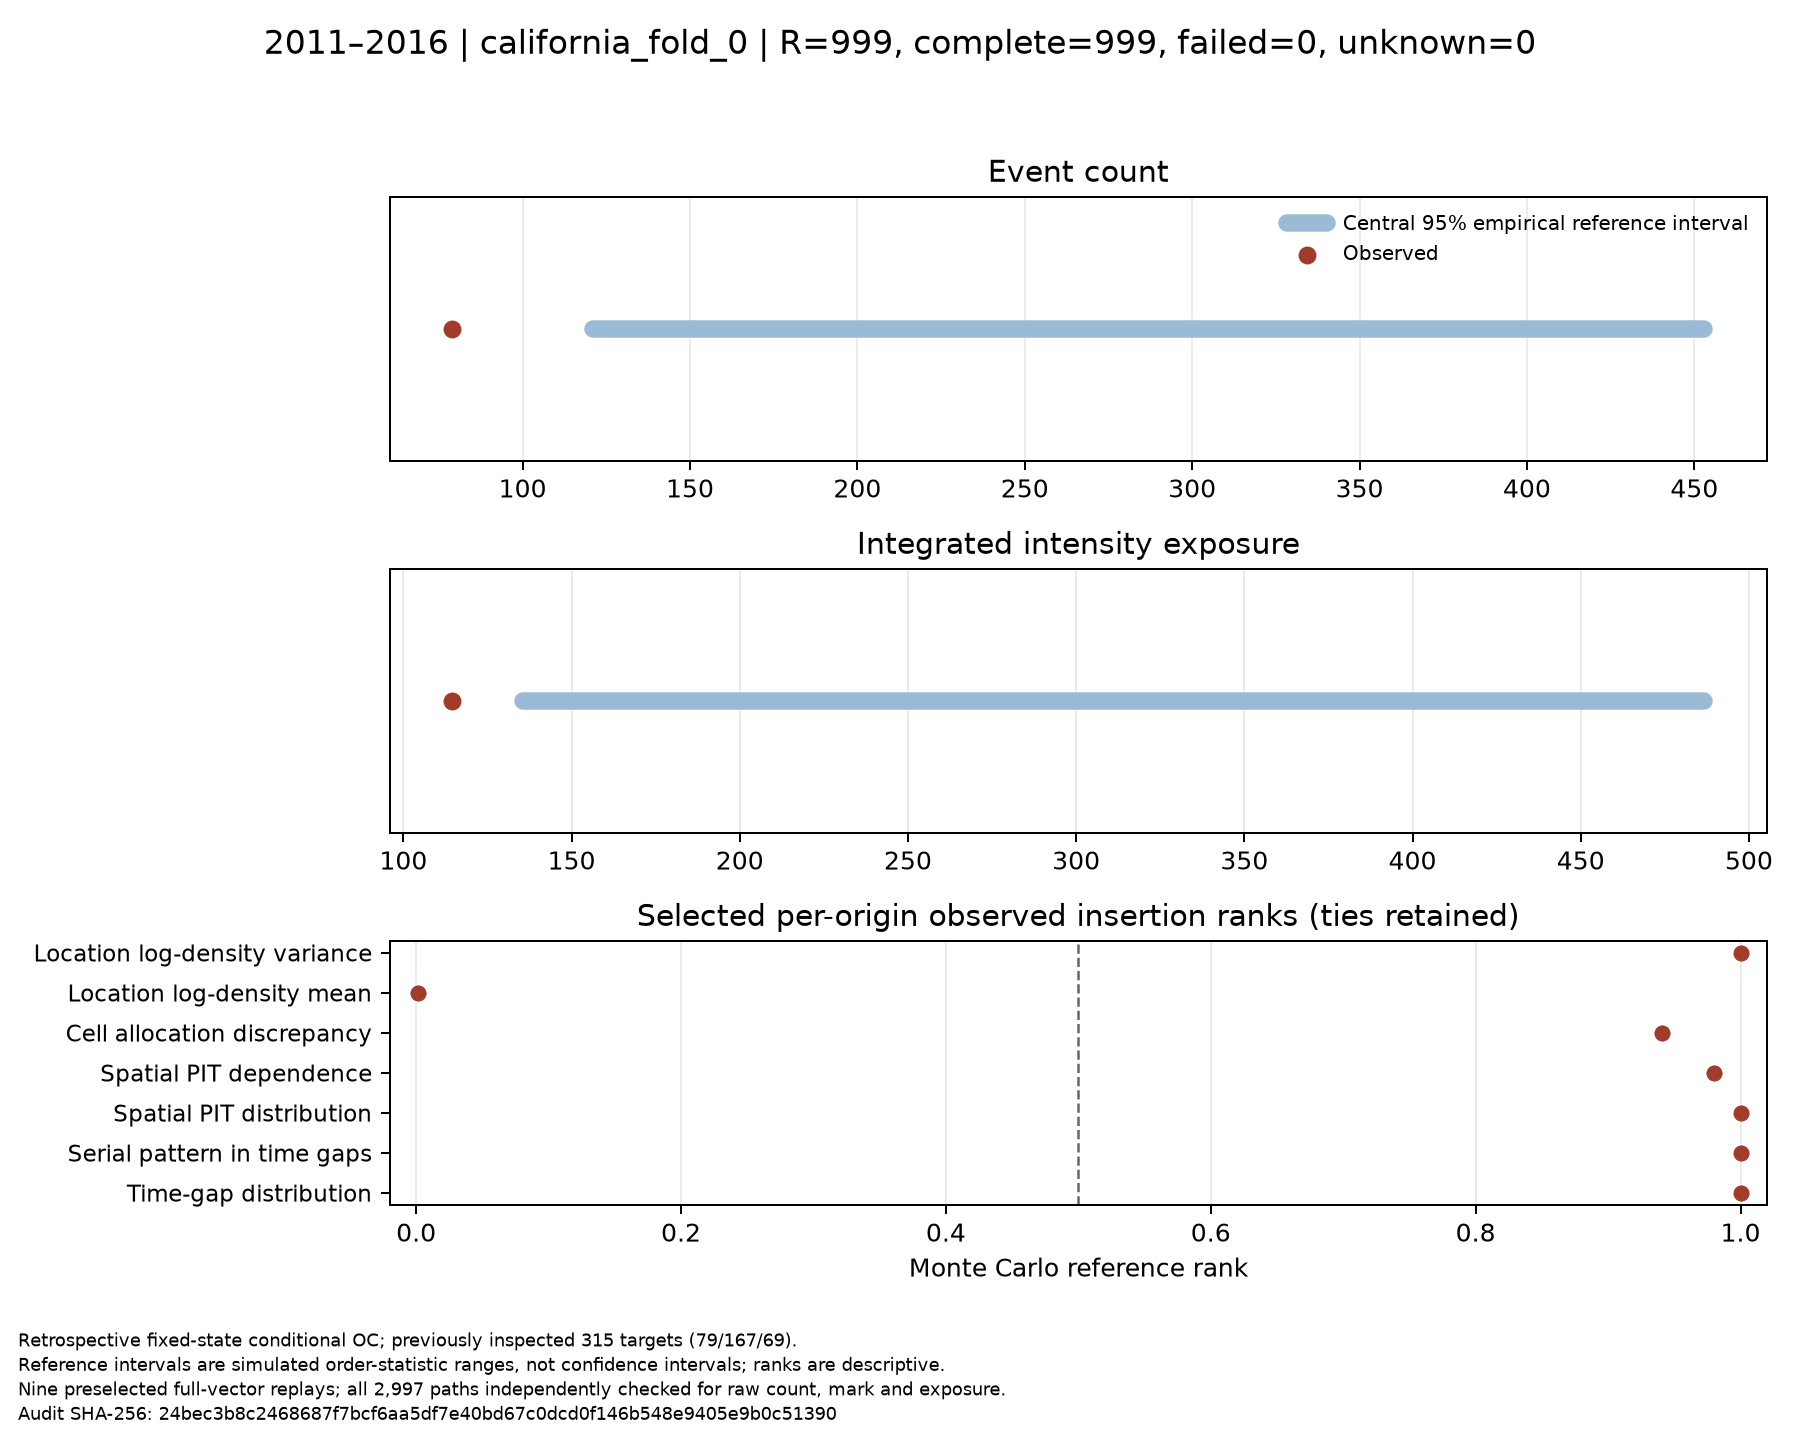
\includegraphics[width=\linewidth,height=.78\textheight,keepaspectratio]{spatial_detail_origin_01.png}
\caption{Conditional diagnostic insertion intervals for frozen OC Fold 0 (2011--2016; 79 observed targets). Immigrant exposure is deterministic; its ties carry no adequacy evidence. Other ties and ordinary-looking coordinates coexist with discrepancies. These are descriptive reference comparisons.}\end{figure}
\clearpage

\clearpage
\begin{figure}[p]\centering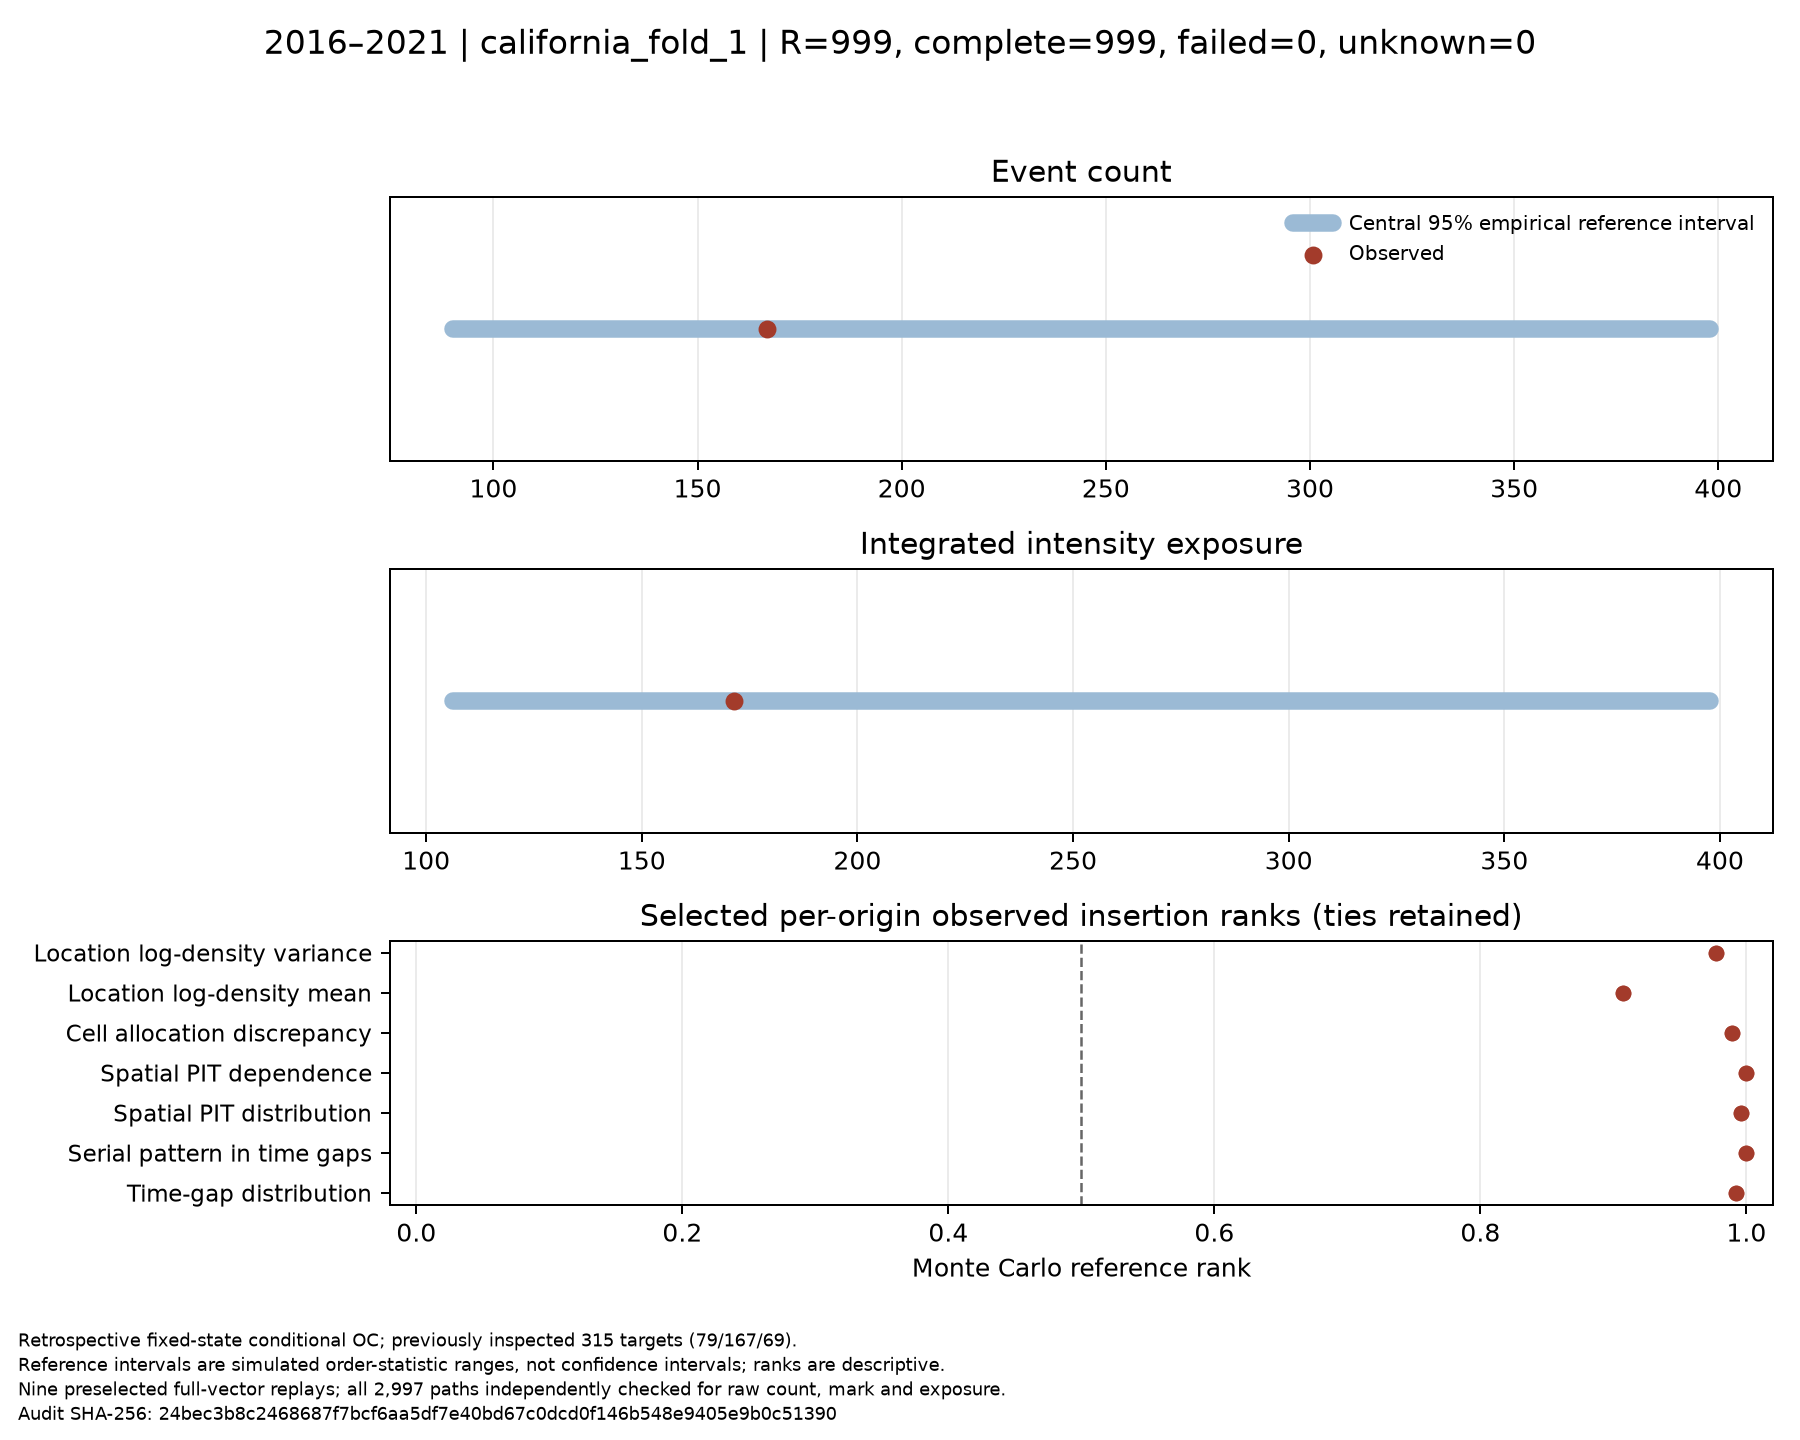
\includegraphics[width=\linewidth,height=.78\textheight,keepaspectratio]{spatial_detail_origin_02.png}
\caption{Conditional diagnostic insertion intervals for frozen OC Fold 1 (2016--2021; 167 observed targets). Immigrant exposure is deterministic; its ties carry no adequacy evidence. Other ties and ordinary-looking coordinates coexist with discrepancies. These are descriptive reference comparisons.}\end{figure}
\clearpage

\clearpage
\begin{figure}[p]\centering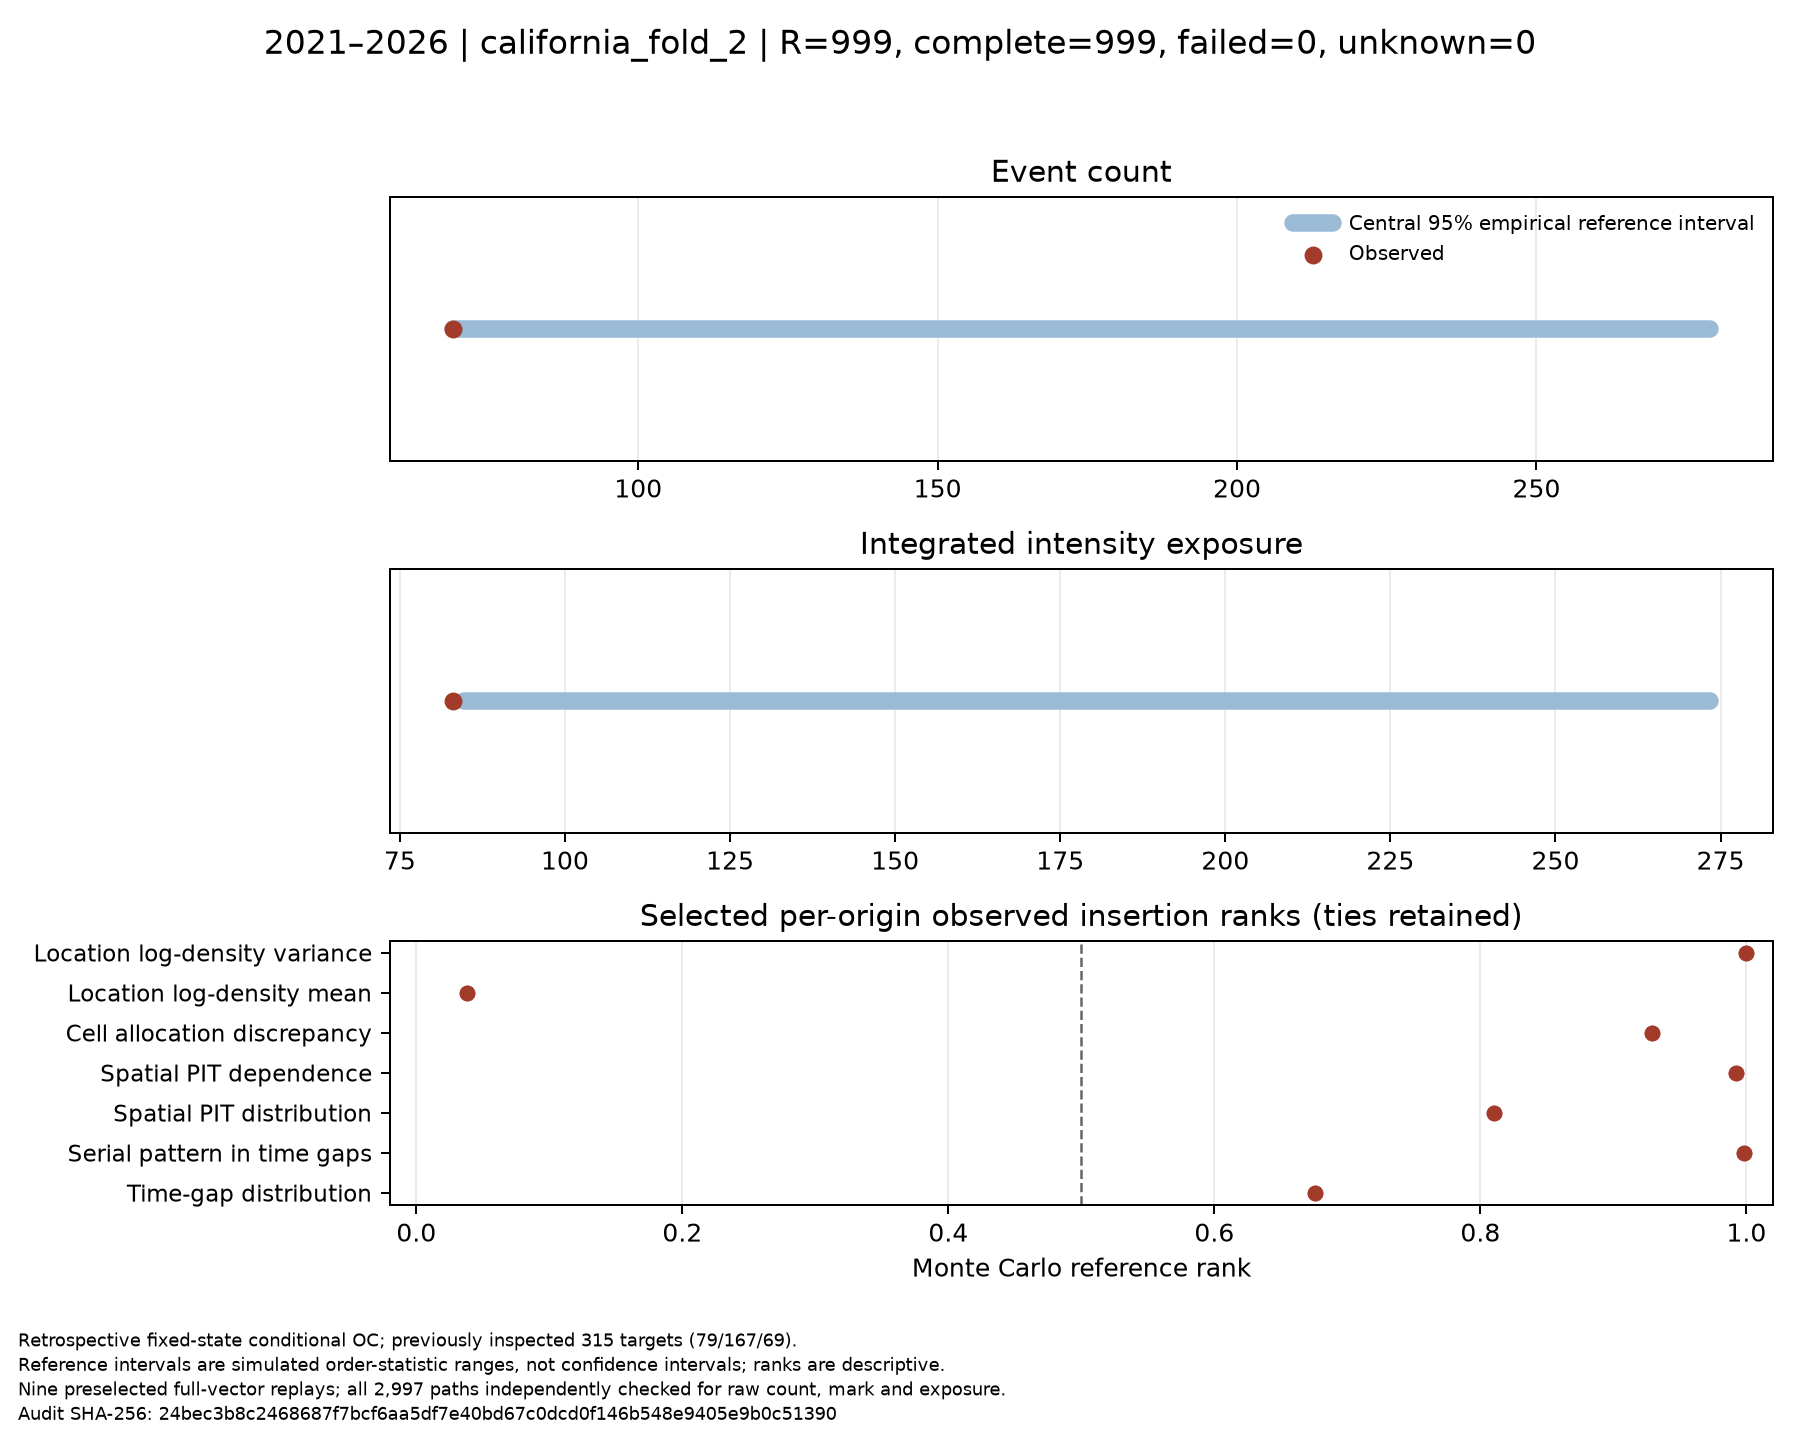
\includegraphics[width=\linewidth,height=.78\textheight,keepaspectratio]{spatial_detail_origin_03.png}
\caption{Conditional diagnostic insertion intervals for frozen OC Fold 2 (2021--2026; 69 observed targets). Immigrant exposure is deterministic; its ties carry no adequacy evidence. Other ties and ordinary-looking coordinates coexist with discrepancies. These are descriptive reference comparisons.}\end{figure}
\clearpage
